%! Author = gramic
%! Date = 26.04.24

% Preamble
\subsection{Patroni}
\label{subsec:evaluation_installation_patroni}
\subsubsection{Prerequisites}
Ganz am Anfang steht die Firewall.\\
Die Rules müssen auf \texttt{sks1232}, \texttt{sks1233}, \texttt{sks1234} und \texttt{sks9016} gesetzt werden:
\lstset{style=gra_codestyle}
\begin{lstlisting}[language=bash, caption=Patroni - Firewall Settings,captionpos=b,label={lst:patroni-firewall-settings},breaklines=true]
# sks1232 / sks1233 / sks1234 / sks9016(10.0.28.16)
nano /etc/iptables/rules.v4
*filter
:INPUT ACCEPT [0:0]
:FORWARD ACCEPT [0:0]
:OUTPUT ACCEPT [0:0]
-A INPUT -s 10.0.0.0/8 -p tcp -m tcp --dport 22 -j ACCEPT
-A INPUT -s 10.0.9.115/32 -p udp -m udp --dport 161 -m comment --comment "Allow SNMP for probe 10.0.9.115" -j ACCEPT
-A INPUT -s 10.0.9.76/32 -p udp -m udp --dport 161 -m comment --comment "Allow SNMP for probe 10.0.9.76" -j ACCEPT
-A INPUT -s 10.0.36.147/32 -p udp -m udp --dport 161 -m comment --comment "Allow SNMP for probe 10.0.36.147" -j ACCEPT
-A INPUT -s 10.0.9.35/32 -p udp -m udp --dport 161 -m comment --comment "Allow SNMP for probe 10.0.9.35" -j ACCEPT
-A INPUT -s 10.0.9.37/32 -p udp -m udp --dport 161 -m comment --comment "Allow SNMP for probe 10.0.9.37" -j ACCEPT
-A INPUT -s 10.0.9.74/32 -p udp -m udp --dport 161 -m comment --comment "Allow SNMP for probe 10.0.9.74" -j ACCEPT
-A INPUT -s 10.0.9.75/32 -p udp -m udp --dport 161 -m comment --comment "Allow SNMP for probe 10.0.9.75" -j ACCEPT
-A INPUT -s 10.0.9.36/32 -p udp -m udp --dport 161 -m comment --comment "Allow SNMP for probe 10.0.9.36" -j ACCEPT
-A INPUT -s 10.0.9.14/32 -p udp -m udp --dport 161 -m comment --comment "Allow SNMP for probe 10.0.9.14" -j ACCEPT
-A INPUT -s 10.0.0.0/8 -p icmp -m icmp --icmp-type 8 -j ACCEPT
# generell
-A INPUT -s 10.0.0.0/8 -p tcp -m tcp --dport 443 -j ACCEPT
# postgres
-A INPUT -s 10.0.0.0/8 -p tcp -m tcp --dport 5432 -j ACCEPT
# patroni
-A INPUT -s 10.0.0.0/8 -p tcp -m tcp --dport 2379 -j ACCEPT
-A INPUT -s 10.0.0.0/8 -p tcp -m tcp --dport 2380 -j ACCEPT
-A INPUT -s 10.0.0.0/8 -p tcp -m tcp --dport 2376 -j ACCEPT
-A INPUT -s 10.0.0.0/8 -p tcp -m tcp --dport 6432 -j ACCEPT
-A INPUT -s 10.0.0.0/8 -p tcp -m tcp --dport 8008 -j ACCEPT
-A INPUT -s 10.0.0.0/8 -p tcp -m tcp --dport 7000 -j ACCEPT
-A INPUT -s 10.0.0.0/8 -p tcp -m tcp --dport 8080 -j ACCEPT
COMMIT
# Completed

systemctl restart iptables
systemctl status iptables
\end{lstlisting}

Danach muss der Proxy gesetzt werden:
\lstset{style=gra_codestyle}
\begin{lstlisting}[language=bash, caption=Patroni - Proxy Settings,captionpos=b,label={lst:patroni-proxy-settings},breaklines=true]
# sks1232 / sks1233 / sks1234
# Proxy setzen
# nano /etc/profile.d/proxy.sh
export https_proxy=http://sproxy.sivc.first-it.ch:8080
export HTTPS_PROXY=http://sproxy.sivc.first-it.ch:8080
export http_proxy=http://sproxy.sivc.first-it.ch:8080
export HTTP_PROXY=http://sproxy.sivc.first-it.ch:8080
export no_proxy=localhost,127.0.0.0/8,::1,10.0.0.0/8,172.16.0.0/12,192.168.0.0/16
export NO_PROXY=localhost,127.0.0.0/8,::1,10.0.0.0/8,172.16.0.0/12,192.168.0.0/16
# source /etc/profile.d/proxy.sh
\end{lstlisting}

Damit das PostgreSQL-Repository eingebunden werden kann,\\
muss dem apt-Proxy gesetzt werden.\\
Da via \Gls{Foreman} Installiert wurde, muss dieser ausgenommen werden:
\lstset{style=gra_codestyle}
\begin{lstlisting}[language=bash, caption=Patroni - apt-Proxy Settings,captionpos=b,label={lst:patroni-apt-proxy-settings},breaklines=true]
# sks1232 / sks1233 / sks1234
# apt-Proxy setzen
# nano /etc/apt/apt.conf.d/proxy.conf
Acauire::http::Proxy "http://sproxy.sivc.first-it.ch:8080";
Acauire::https::Proxy "http://sproxy.sivc.first-it.ch:8080";
Acquire::http::proxy::foreman.ksgr.ch "DIRECT";
\end{lstlisting}

Im nächsten Schritt kann das PostgreSQL-Repository eingebunden werden.
\begin{warning}
Achtung, die von PostgreSQL beschriebene Variante wurde in Debian 10 als Deprecated gesetzt,
mit Debian 13 wird diese Repository-Integration einen Fehler werden.
\end{warning}

\lstset{style=gra_codestyle}
\begin{lstlisting}[language=bash, caption=Patroni - PostgreSQL einbinden,captionpos=b,label={lst:patroni-include-repository},breaklines=true]
# sks1232 / sks1233 / sks1234
# PostgreSQL Repository einbinden
sudo sh -c 'echo "deb https://apt.postgresql.org/pub/repos/apt $(lsb_release -cs)-pgdg main" > /etc/apt/sources.list.d/pgdg.list'
wget --quiet -O - https://www.postgresql.org/media/keys/ACCC4CF8.asc | sudo apt-key add -

# Ausloggen und wieder einloggen
apt update
\end{lstlisting}

Nun muss der \Gls{PostgreSQL Cluster}, Patroni, python3-etcd und python3-psycopg2 installiert werden:
\lstset{style=gra_codestyle}
\begin{lstlisting}[language=bash, caption=Patroni - Prerequisites installieren,captionpos=b,label={lst:patroni-prerequisites-install},breaklines=true]
apt install postgresql-16 postgresql-server-dev-16 patroni python3-etcd python3-psycopg2
\end{lstlisting}

Im nächsten Schritt müssen Patroni und der \Gls{PostgreSQL Cluster} gestoppt werden:
\lstset{style=gra_codestyle}
\begin{lstlisting}[language=bash, caption=Patroni - Stop Patroni und PostgreSQL,captionpos=b,label={lst:patroni-stop-postgresql-patroni},breaklines=true]
systemctl stop postgresql patroni
\end{lstlisting}

Anschliessend muss noch vom PostgreSQL-Verzeichnis \texttt{/usr/lib/postgresql/16/bin/} ein Symlink nach \texttt{/usr/sbin/} gesetzt werden:
\lstset{style=gra_codestyle}
\begin{lstlisting}[language=bash, caption=Patroni - Symlink binaries,captionpos=b,label={lst:patroni_symlink_bins},breaklines=true]
ln -s /usr/lib/postgresql/16/bin/* /usr/sbin/
\end{lstlisting}

Zu guter Letzt sollte geprüft werden, ob alle Versionen passen und am richtigen Ort sind:
\lstset{style=gra_codestyle}
\begin{lstlisting}[language=bash, caption=Patroni - Checks,captionpos=b,label={lst:patroni-checks},breaklines=true]
which patroni
which psql
patroni --version
\end{lstlisting}
Damit kann zum \gls{etcd} übergegangen werden.

\subsubsection{Installation etcd}
Auf \texttt{sks9016} sollte erst das Repository angepasst werden und anschliessend der \texttt{etcd-server} installiert werden:
\lstset{style=gra_codestyle}
\begin{lstlisting}[language=bash, caption=etcd - Installation,captionpos=b,label={lst:etcd_install},breaklines=true]
apt update
apt install etcd-server
\end{lstlisting}

Die Konfiguration ist simpel.\\
Die IP muss gesetzt werden, ein Listener auf Localhost und IP gesetzt werden:
\lstset{style=gra_codestyle}
\begin{lstlisting}[language=bash, caption=etcd - Konfiguration,captionpos=b,label={lst:etcd_configuration},breaklines=true]
# nano /etc/default/etcd
ETCD_LISTEN_PEER_URLS="http://10.0.28.16:2380"
ETCD_LISTEN_CLIENT_URLS="http://localhost:2379,http://10.0.28.16:2379"
ETCD_INITIAL_ADVERTISE_PEER_URLS="http://10.0.28.16:2380"
ETCD_INITIAL_CLUSTER="default=http://10.0.28.16:2380,"
ETCD_ADVERTISE_CLIENT_URLS="http://10.0.28.16:2379"
ETCD_INITIAL_CLUSTER_TOKEN="etcd-cluster"
ETCD_INITIAL_CLUSTER_STATE="new"
\end{lstlisting}

Der Service sollte neu gestartet und seine lauffähigkeit getestet werden:
\lstset{style=gra_codestyle}
\begin{lstlisting}[language=bash, caption=etcd - restart,captionpos=b,label={lst:etcd_restart},breaklines=true]
systemctl restart etcd
systemctl is-enabled etcd
systemctl status etcd
\end{lstlisting}

Es sollte nun ein Member gelistet werden:
\lstset{style=gra_codestyle}
\begin{lstlisting}[language=bash, caption=etcd - member list,captionpos=b,label={lst:etcd_member_list},breaklines=true]
etcdctl member list
\end{lstlisting}

Damit kann nun das Bootstrapping gestartet werden.

\subsubsection{Bootstrapping}
Zuerst müssen die yml-Konfigurationen gesetzt werden.\\
Am besten wird das bestehende File jeweils gelöscht:
\lstset{style=gra_codestyle}
\begin{lstlisting}[language=bash, caption=Patroni Bootstrap - Konfiguration bereinigen,captionpos=b,label={lst:patroni-bootstrap-cleanup-yml},breaklines=true]
rm /etc/patroni/config.yml
nano /etc/patroni/config.yml
\end{lstlisting}

Die yml-Files sehen wie folgt aus:
\lstset{style=gra_codestyle}
\begin{lstlisting}[language=yaml, caption=Patroni - Konfiguration - sks1232,captionpos=b,label={lst:sks1232_patroni.yml},breaklines=true]
# Scope of PostgreSQL
scope: postgres
# Namespace for the PostgreSQL database
namespace: /db/
# Name of the PostgreSQL instance
name: postgres01
# Patroni REST API Configuration
restapi:
    # The IP address and port on which the REST API should listen
    listen: 10.0.20.110:8008

    # The IP address and port to which clients should connect
    connect_address: 10.0.20.110:8008
# Patroni Etcd Configuration
etcd3:
    # The host address and port of the Etcd server
    host: 10.0.28.16:2379
# Patroni Bootstrap Configuration
bootstrap:
    # Configuration parameters for distributed configuration store (DCS)
    dcs:
        ttl: 30
        loop_wait: 10
        retry_timeout: 10
        maximum_lag_on_failover: 1048576
        postgresql:
            # Use pg_rewind during bootstrap
            use_pg_rewind: true
            #   Change pg_wal
            create_replica_methods:
                - basebackup
            basebackup:
                max-rate: '100M'
                waldir: "/srv/data/pg_wal"
    # Initdb configuration
    # Initdb configuration
    initdb:
        - auth: scram-sha-256
        - encoding: UTF8
        - data-checksums
    # pg_hba.conf entries for replication and general access
    pg_hba:
        - host replication replicator 127.0.0.1/32 scram-sha-256
        - host replication replicator 10.0.20.110/0 scram-sha-256
        - host replication replicator 10.0.20.111/0 scram-sha-256
        - host replication replicator 10.0.20.112/0 scram-sha-256
        - host all all 0.0.0.0/0 scram-sha-256
    # Adding default user admin with password admin
    users:
      admin:
          password: admin
          options:
              - createrole
              - createdb
# Patroni PostgreSQL Configuration
postgresql:
    # PostgreSQL server listening address and port
    listen: 10.0.20.110:5432
    # Connect address for PostgreSQL clients
    connect_address: 10.0.20.110:5432
    # Data directory for PostgreSQL
    data_dir: /var/lib/patroni
    # Path to the pgpass file
    pgpass: /tmp/pgpass
    # Authentication configuration
    authentication:
        # Replication of user credentials
        replication:
            username: replicator
            password: replicator
        # Superuser credentials
        superuser:
            username: postgres
            password: postgres
    # Additional PostgreSQL parameters
    parameters:

        # Directory for Unix socket
        unix_socket_directories: '.'
        # Password encryption method
        password_encryption: 'scram-sha-256'
# Patroni Tags Configuration
tags:
    # Prevents a node from being promoted in case of failure
    nofailover: false
    # Prevents the load balancer from considering this node
    noloadbalance: false
    # Prevents a replica from being created by cloning
    clonefrom: false
    # Prevents synchronous replication from being enforced
    nosync: false

\end{lstlisting}

\lstset{style=gra_codestyle}
\begin{lstlisting}[language=yaml, caption=Patroni - Konfiguration - sks1233,captionpos=b,label={lst:sks1233_patroni.yml},breaklines=true]
# Scope of PostgreSQL
scope: postgres
# Namespace for the PostgreSQL database
namespace: /db/
# Name of the PostgreSQL instance
name: postgres02
# Patroni REST API Configuration
restapi:
    # The IP address and port on which the REST API should listen
    listen: 10.0.20.111:8008

    # The IP address and port to which clients should connect
    connect_address: 10.0.20.111:8008
# Patroni Etcd Configuration
etcd3:
    # The host address and port of the Etcd server
    host: 10.0.28.16:2379
# Patroni Bootstrap Configuration
bootstrap:
    # Configuration parameters for distributed configuration store (DCS)
    dcs:
        ttl: 30
        loop_wait: 10
        retry_timeout: 10
        maximum_lag_on_failover: 1048576
        postgresql:
            # Use pg_rewind during bootstrap
            use_pg_rewind: true
            #   Change pg_wal
            create_replica_methods:
                - basebackup
            basebackup:
                max-rate: '100M'
                waldir: "/srv/data/pg_wal"
    # Initdb configuration
    # Initdb configuration
    initdb:
        - auth: scram-sha-256
        - encoding: UTF8
        - data-checksums
    # pg_hba.conf entries for replication and general access
    pg_hba:
        - host replication replicator 127.0.0.1/32 scram-sha-256
        - host replication replicator 10.0.20.110/0 scram-sha-256
        - host replication replicator 10.0.20.111/0 scram-sha-256
        - host replication replicator 10.0.20.112/0 scram-sha-256
        - host all all 0.0.0.0/0 scram-sha-256
    # Adding default user admin with password admin
    users:
      admin:
          password: admin
          options:
              - createrole
              - createdb
# Patroni PostgreSQL Configuration
postgresql:
    # PostgreSQL server listening address and port
    listen: 10.0.20.111:5432
    # Connect address for PostgreSQL clients
    connect_address: 10.0.20.111:5432
    # Data directory for PostgreSQL
    data_dir: /var/lib/patroni
    # Path to the pgpass file
    pgpass: /tmp/pgpass

    # Authentication configuration
    authentication:
        # Replication of user credentials
        replication:
            username: replicator
            password: replicator
        # Superuser credentials
        superuser:
            username: postgres
            password: postgres
    # Additional PostgreSQL parameters
    parameters:
        # Directory for Unix socket
        unix_socket_directories: '.'
        # Password encryption method
        password_encryption: 'scram-sha-256'
# Patroni Tags Configuration
tags:
    # Prevents a node from being promoted in case of failure
    nofailover: false
    # Prevents the load balancer from considering this node
    noloadbalance: false
    # Prevents a replica from being created by cloning
    clonefrom: false
    # Prevents synchronous replication from being enforced
    nosync: false

\end{lstlisting}

\lstset{style=gra_codestyle}
\begin{lstlisting}[language=yaml, caption=Patroni - Konfiguration - sks1234,captionpos=b,label={lst:sks1234_patroni.yml},breaklines=true]
# Scope of PostgreSQL
scope: postgres
# Namespace for the PostgreSQL database
namespace: /db/
# Name of the PostgreSQL instance
name: postgres03
# Patroni REST API Configuration
restapi:
    # The IP address and port on which the REST API should listen
    listen: 10.0.20.112:8008

    # The IP address and port to which clients should connect
    connect_address: 10.0.20.112:8008
# Patroni Etcd Configuration
etcd3:
    # The host address and port of the Etcd server
    host: 10.0.28.16:2379
# Patroni Bootstrap Configuration
bootstrap:
    # Configuration parameters for distributed configuration store (DCS)
    dcs:
        ttl: 30
        loop_wait: 10
        retry_timeout: 10
        maximum_lag_on_failover: 1048576
        postgresql:
            # Use pg_rewind during bootstrap
            use_pg_rewind: true
            #   Change pg_wal
            create_replica_methods:
                - basebackup
            basebackup:
                max-rate: '100M'
                waldir: "/srv/data/pg_wal"
    # Initdb configuration
    initdb:
        - auth: scram-sha-256
        - encoding: UTF8
        - data-checksums
    # pg_hba.conf entries for replication and general access
    pg_hba:
        - host replication replicator 127.0.0.1/32 scram-sha-256
        - host replication replicator 10.0.20.110/0 scram-sha-256
        - host replication replicator 10.0.20.111/0 scram-sha-256
        - host replication replicator 10.0.20.112/0 scram-sha-256
        - host all all 0.0.0.0/0 scram-sha-256
    # Adding default user admin with password admin
    users:
      admin:
          password: admin
          options:
              - createrole
              - createdb
# Patroni PostgreSQL Configuration
postgresql:
    # PostgreSQL server listening address and port
    listen: 10.0.20.112:5432
    # Connect address for PostgreSQL clients
    connect_address: 10.0.20.112:5432
    # Data directory for PostgreSQL
    data_dir: /var/lib/patroni
    # Path to the pgpass file
    pgpass: /tmp/pgpass
    # Authentication configuration
    authentication:
        # Replication of user credentials
        replication:
            username: replicator
            password: replicator
        # Superuser credentials
        superuser:
            username: postgres
            password: postgres
    # Additional PostgreSQL parameters
    parameters:
        unix_socket_directories: '.'
        # Password encryption method
        password_encryption: 'scram-sha-256'
# Patroni Tags Configuration
tags:
    # Prevents a node from being promoted in case of failure
    nofailover: false
    # Prevents the load balancer from considering this node
    noloadbalance: false
    # Prevents a replica from being created by cloning
    clonefrom: false
    # Prevents synchronous replication from being enforced
    nosync: false

\end{lstlisting}

Sehr wichtig ist, dass das \texttt{pg\_hba.conf}-File mitgegeben wird.\\
Ansonsten kann nicht auf die Datenbank zugegriffen werden.\\
Für den User \texttt{replication} müssen die IP-Adressen aller Nodes gesetzt werden.\\
Im Evaluations-Enviroment soll zudem der Zugriff von überall mit Passwort möglich sein.\\
Dies wird mit der letzten Zeile ermöglicht:
\lstset{style=gra_codestyle}
\begin{lstlisting}[language=bash, caption=Patroni Bootstrap - pg\_hba,captionpos=b,label={lst:patroni-pg_hba},breaklines=true]
host replication replicator 127.0.0.1/32 scram-sha-256
host replication replicator 10.0.20.110/0 scram-sha-256
host replication replicator 10.0.20.111/0 scram-sha-256
host replication replicator 10.0.20.112/0 scram-sha-256
host all all 0.0.0.0/0 scram-sha-256
\end{lstlisting}

Nun muss das Verzeichnis für PostgreSQL im Patroni-Verzeichnis erstellt und berechtigt werden:
\lstset{style=gra_codestyle}
\begin{lstlisting}[language=bash, caption=Patroni Bootstrap - Patroni-Verzeichnis,captionpos=b,label={lst:patroni-directory},breaklines=true]
mkdir -p /var/lib/patroni
chown -R postgres:postgres /var/lib/patroni
chmod 700 /var/lib/patroni
\end{lstlisting}

Jetzt können die Dienste auf den Patroni-Servern neu gestartet werden, Patroni sollte nun lauffähig sein:
\lstset{style=gra_codestyle}
\begin{lstlisting}[language=bash, caption=Patroni Bootstrap - Neu starten,captionpos=b,label={lst:patroni-restart},breaklines=true]
systemctl start patroni
systemctl status patroni
patronictl -c /etc/patroni/config.yml list
\end{lstlisting}

Wenn es lauffähig ist, muss noch aufgeräumt werden.\\
Der bestehende \Gls{PostgreSQL Cluster} muss disabled werden:
\lstset{style=gra_codestyle}
\begin{lstlisting}[language=bash, caption=Patroni Bootstrap - Disable PostgreSQL,captionpos=b,label={lst:patroni-disable-postgresql},breaklines=true]
sudo systemctl disable --now postgresql
\end{lstlisting}

\subsubsection{HAproxy}
Final kann nun HAproxy installiert werden.\\
Zuerst müssen die Hosts hinterlegt werden:
\lstset{style=gra_codestyle}
\begin{lstlisting}[language=bash, caption=HAproxy - Hostliste,captionpos=b,label={lst:haproxy_hostlist},breaklines=true]
#nano /etc/hosts
10.0.20.110    postgres01
10.0.20.111    postgres02
10.0.20.112    postgres03
\end{lstlisting}

Nun müssen die Repositories aktualisiert werden und HAproxy installiert werden:
\lstset{style=gra_codestyle}
\begin{lstlisting}[language=bash, caption=HAproxy - Installation,captionpos=b,label={lst:haproxy_installation},breaklines=true]
apt update
apt install haproxy
\end{lstlisting}

Mit der Installation kommt ein Konfig-File mit.\\
Das soll gesichert werden:
\lstset{style=gra_codestyle}
\begin{lstlisting}[language=bash, caption=HAproxy - Safe Alte Config,captionpos=b,label={lst:haproxy_safe_old_config},breaklines=true]
mv /etc/haproxy/haproxy.cfg /etc/haproxy/haproxy.cfg.orig
\end{lstlisting}

Nun muss die neue Konfiguration geschrieben werden:
\lstset{style=gra_codestyle}
\begin{lstlisting}[language=bash, caption=HAproxy - Konfiguration,captionpos=b,label={lst:haproxy_config},breaklines=true]
#nano /etc/haproxy/haproxy.cfg
# Global configuration settings
global
    # Maximum connections globally
    maxconn 100
    # Logging settings
    log 127.0.0.1 local2

# Default settings
defaults
    # Global log configuration
    log global
    # Set mode to TCP
    mode tcp
    # Number of retries
    retries 2
    # Client timeout
    timeout client 30m
    # Connect timeout
    timeout connect 4s
    # Server timeout
    timeout server 30m
    # Check timeout
    timeout check 5s

# Stats configuration
listen stats
    # Set mode to HTTP
    mode http
    # Bind to port 8080
    bind *:8080
    # Enable stats
    stats enable
    # Stats URI
    stats uri /

# PostgreSQL configuration
listen postgres
    # Bind to port 5432
    bind *:5432
    # Enable HTTP check
    option httpchk
    # Expect status 200
    http-check expect status 200
    # Server settings
    default-server inter 3s fall 3 rise 2 on-marked-down shutdown-sessions
    # Define PostgreSQL servers
    server postgres01 10.0.20.110:5432 maxconn 100 check port 8008
    server postgres02 10.0.20.111:5432 maxconn 100 check port 8008
    server postgres03 10.0.20.112:5432 maxconn 100 check port 8008
\end{lstlisting}

Nun kann HAproxy neu gestartet werden:
\lstset{style=gra_codestyle}
\begin{lstlisting}[language=bash, caption=HAproxy - Restart,captionpos=b,label={lst:haproxy_restart},breaklines=true]
systemctl restart haproxy
systemctl status haproxy
\end{lstlisting}

Nun kann HAproxy geöffnet werden:
\url{http://10.0.28.16:8080/}

Es sollte nun so aussehen:
\begin{figure}[H]
    \centering
    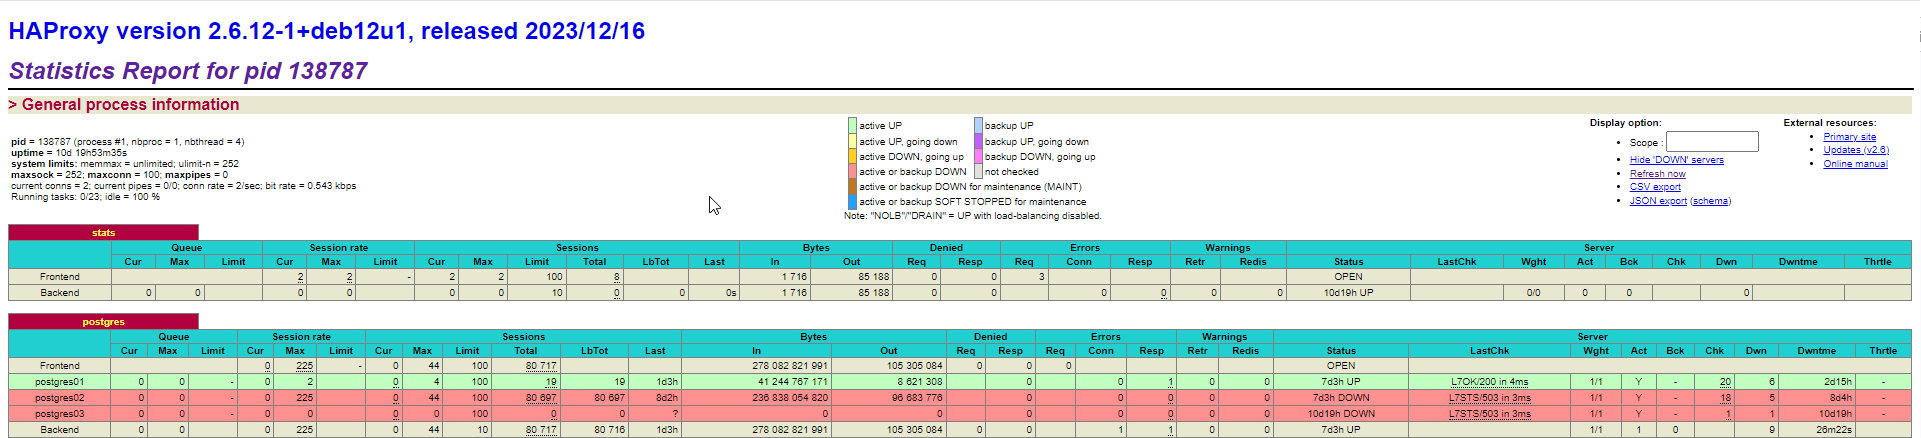
\includegraphics[width=0.8\linewidth]{source/implementation/evaluation/postgresql_ha_solutions/patroni/haproxy_webgui}
    \caption{HAproxy - Web-GUI}
    \label{fig:haproxy-webgui}
\end{figure}

\subsubsection{Installation - 250GiB}
